\section{Results}
\label{sec:results}
%NOTE the following graphs do not have autogluon in it but it is built in my code, im just testing my analysis pipeline with "dummy data" - models trained on 1 epoch for fast result collection
The results can be categorized into four seperate splits: ($t+6$, phases),($t+6$, no-phases), ($t+12$, phases), and ($t+12$, no-phases)
These categories are distinct and can not be compared to each other. It is only appropriate to compare models within the categories.
\subsection{Bootstrap}

After training and testing on each boostrap dataset we are able to obtain the behavior of a model by collecting their metrics for every bootstrap dataset.

\begin{figure}[H]
    \centering
    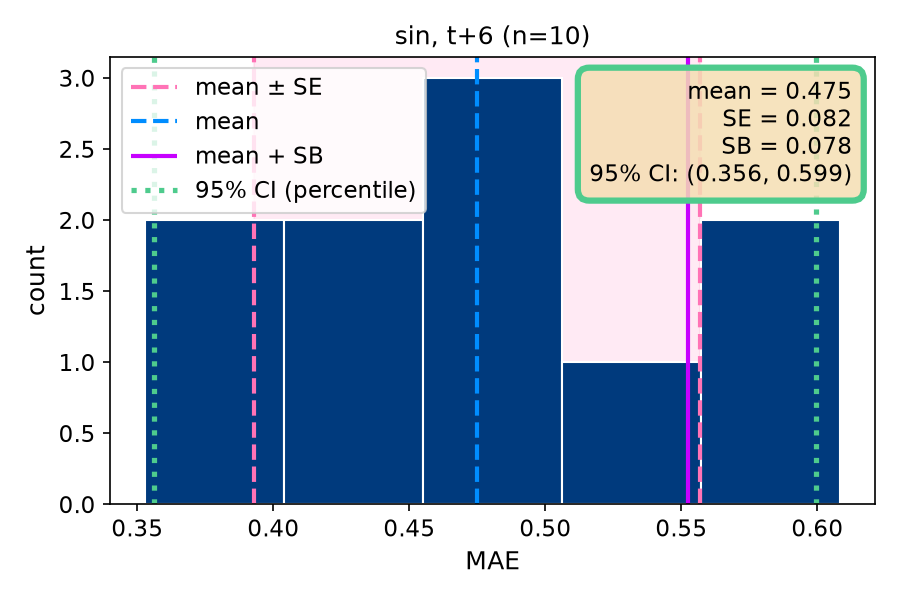
\includegraphics[width=0.7\textwidth]{figs/results/bootstrap/mae_sin_t+6_phases.png}
    \caption{MAE of the sinusoidal transformer at $t+6$ (30 minutes) on each of the 10 bootstrap datasets (seeds averaged per dataset), with the mean, mean $\pm$ SE and the 95\% percentile interval.}
    \label{fig:bootstrap_mae_sin_t6}
\end{figure}
\subsubsection{Training Time}
\begin{figure}[H]
    \centering
    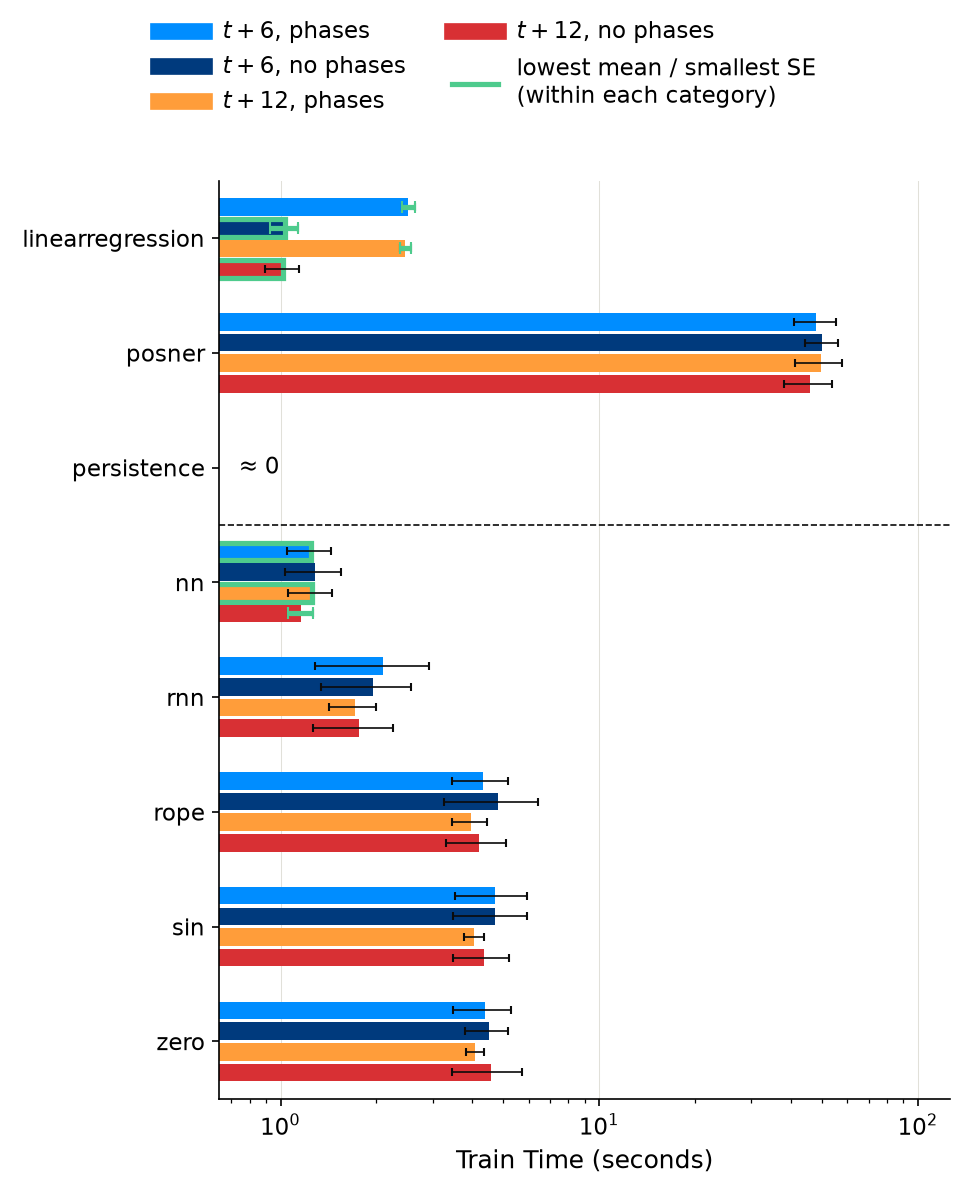
\includegraphics[width=0.7\textwidth]{figs/results/bootstrap/train_time_bars_grouped.png}
    \caption{Mean training time of every model over the 10 bootstrap datasets, one bar per forecast horizon and phase setting, with bootstrap standard error bars. Baselines are above the dashed line and champions below it. Green marks the lowest mean (outline) and smallest standard error (error bar) within each category.}
    \label{fig:bootstrap_mae_boxplot}
\end{figure}
\subsubsection{MAE}
The mean and variance of the models metrics from every dataset tells us the effectiveness of the model predictions in a category.
We can then compare the models forecast metrics with a side by side comparison.
\begin{figure}[H]
    \centering
    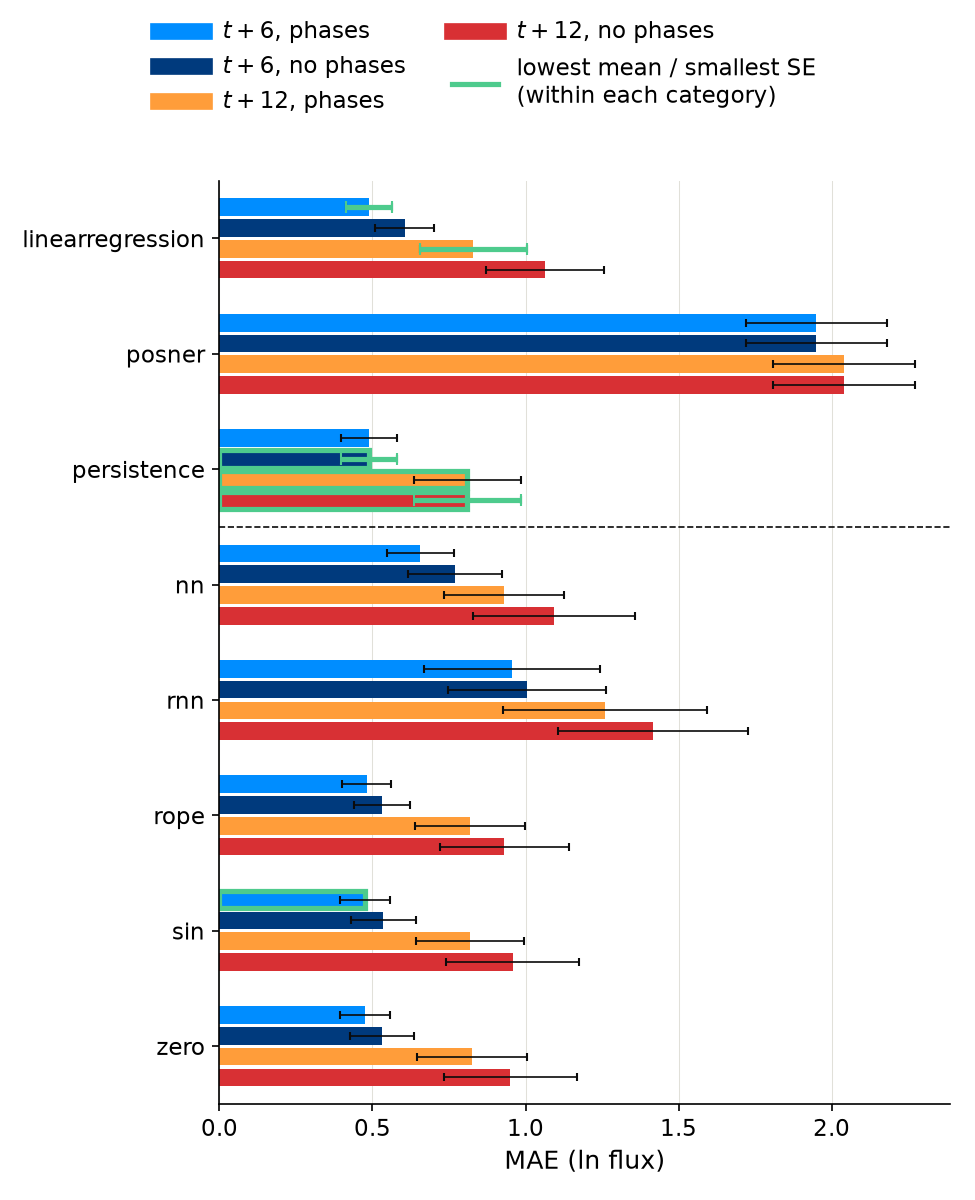
\includegraphics[width=0.7\textwidth]{figs/results/bootstrap/mae_bars_grouped.png}
    \caption{Mean MAE of every model over the 10 bootstrap datasets, one bar per forecast horizon and phase setting, with bootstrap standard error bars. Baselines are above the dashed line and champions below it. Green marks the lowest mean (outline) and smallest standard error (error bar) within each category.}
    \label{fig:bootstrap_mae_bars}
\end{figure}
For ($t+6$, phases) the model with the lowest MAE of XXXX is from model XXXXXX with a standard error of XXXXX. YYYYY had the lowest standard error of YYYYY. 
($t+6$, no-phases) model with the lowest mean MAE was YYY with smallest stanard error model YYY.
($t+12$, phases) lowest mean MAE is ZZZ with smallest standard error ZZZ
($t+12$, no-phases) lowest mean MAE is WWW with smallest standard error WWW
\textit{Stuff here on why i think the winning models are who they are. Confirm that the NN, RNN, Posner, Persistent models matches Torres models under same parameters}

\begin{figure}[H]
    \centering
    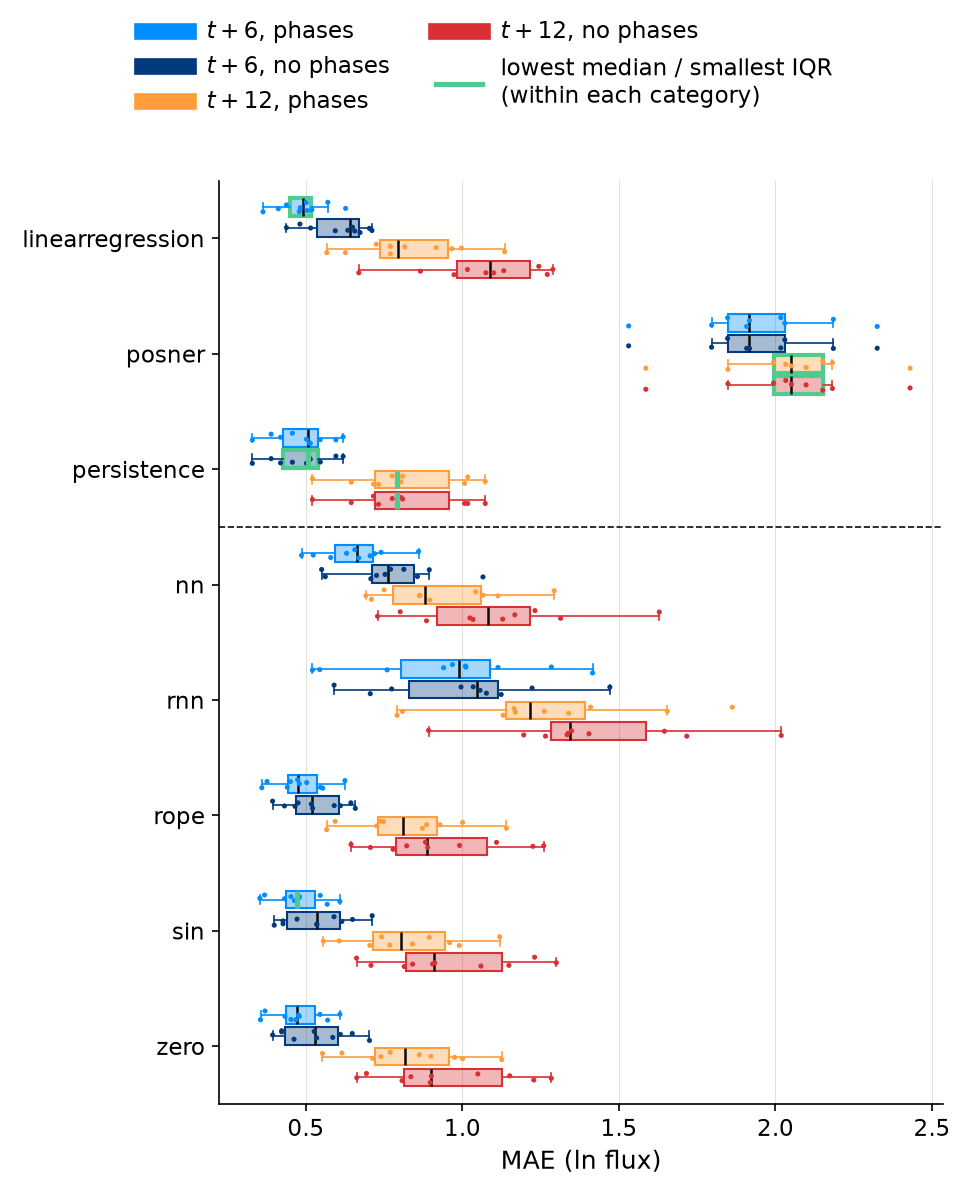
\includegraphics[width=0.7\textwidth]{figs/results/bootstrap/mae_boxplot_grouped.png}
    \caption{MAE of every model on the 10 bootstrap datasets (seeds averaged per dataset), one box per forecast horizon and phase setting. Baselines are above the dashed line and champions below it. Green marks the lowest median (line) and smallest interquartile range (box outline) within each category.}
    \label{fig:bootstrap_mae_boxplot}
\end{figure}

\subsubsection{Lag}
We duplicate the visual check with the lag values. we perform our analysis on the onset to peak lags.

\begin{figure}[H]
    \centering
    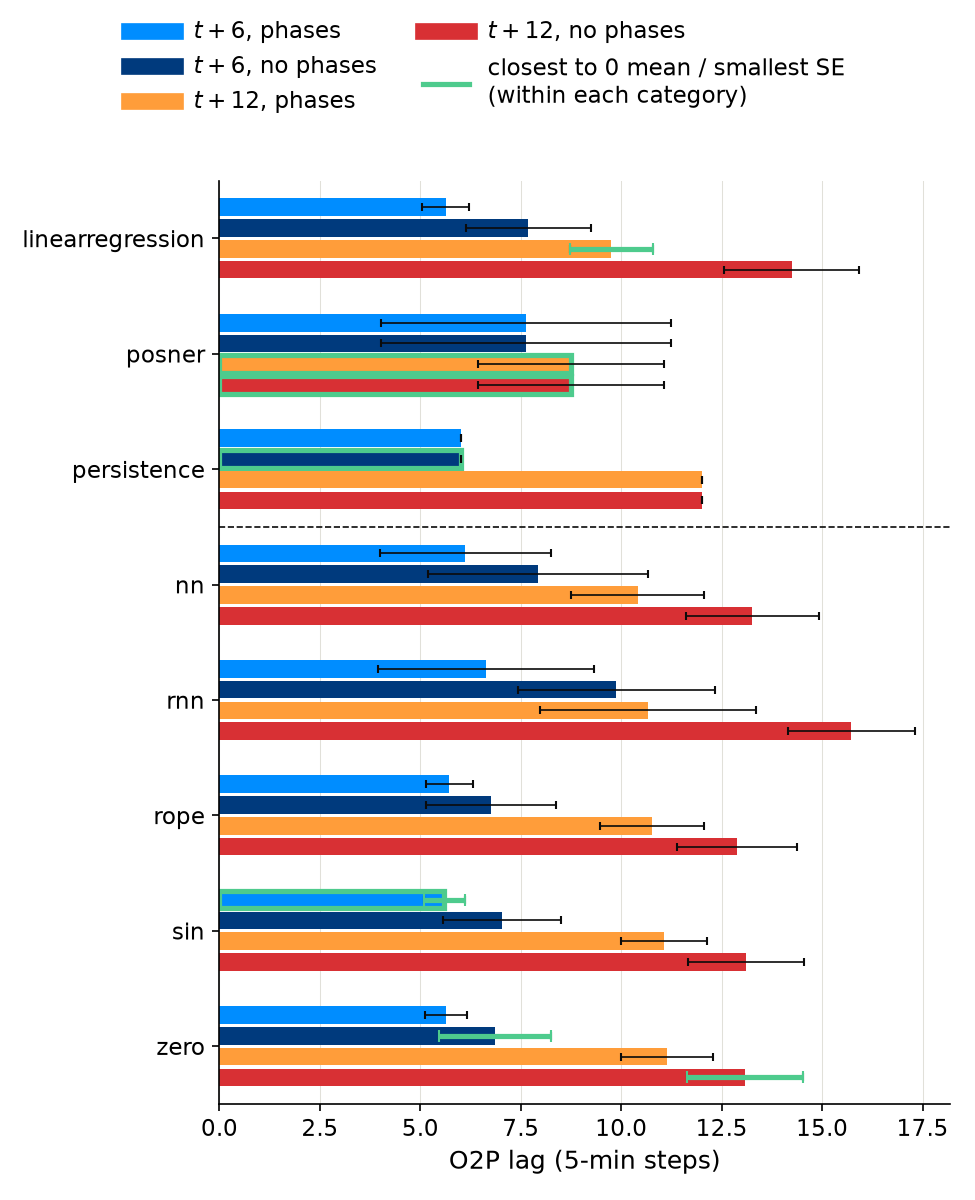
\includegraphics[width=0.7\textwidth]{figs/results/bootstrap/o2p_lag_bars_grouped.png}
    \caption{Mean onset-to-peak (O2P) lag of every model over the 10 bootstrap datasets, in 5-minute steps, one bar per forecast horizon and phase setting, with bootstrap standard error bars. Baselines are above the dashed line and champions below it. Green marks the mean closest to zero (outline) and smallest standard error (error bar) within each category}
    \label{fig:bootstrap_o2p_lag_bars}
\end{figure}
Posner overpredicts the rise in forecast with values $LLL \pm LL$. Persistence will always have an O2P lag of $6.0$ and $12.0$ for $(t+6, t+12)$ respectively, regardless of the flux dataset.
This means that the spread will always be zero. For ($t+6$, phases) the model with the lowest O2P Lag of XXXX is from model XXXXXX with a standard error of XXXXX. YYYYY had the lowest standard error of YYYYY. 
($t+6$, no-phases) model with the lowest mean O2P Lag was YYY with smallest stanard error model YYY.
($t+12$, phases) lowest mean O2P Lag is ZZZ with smallest standard error ZZZ
($t+12$, no-phases) lowest mean O2P Lag is WWW with smallest standard error WWW
\textit{Stuff here on why i think the winning models are who they are. Confirm that the NN, RNN, Posner, Persistent models matches Torres models under same parameters}

\begin{figure}[H]
    \centering
    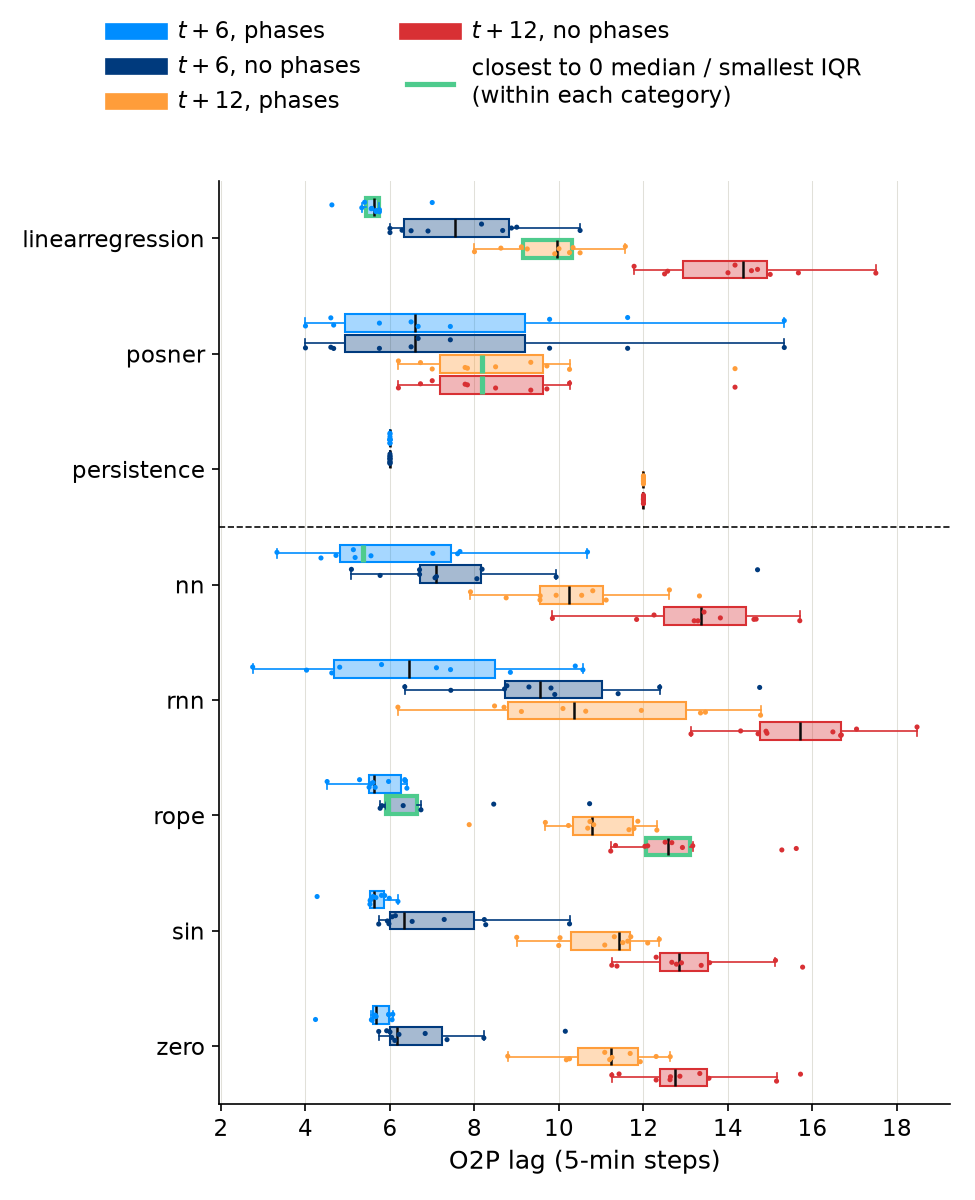
\includegraphics[width=0.7\textwidth]{figs/results/bootstrap/o2p_lag_boxplot_grouped.png}
    \caption{Onset-to-peak (O2P) lag of every model on the 10 bootstrap datasets (seeds averaged per dataset), in 5-minute steps, one box per forecast horizon and phase setting. Baselines are above the dashed line and champions below it. Green marks the median closest to zero (line) and smallest interquartile range (box outline) within each category.}
    \label{fig:bootstrap_o2p_lag_boxplot}
\end{figure}
\subsubsection{Correlation}
We repeat the comparison with the prediction efficiency (PE), where higher is better and a PE of $1$ is a perfect forecast.

\begin{figure}[H]
    \centering
    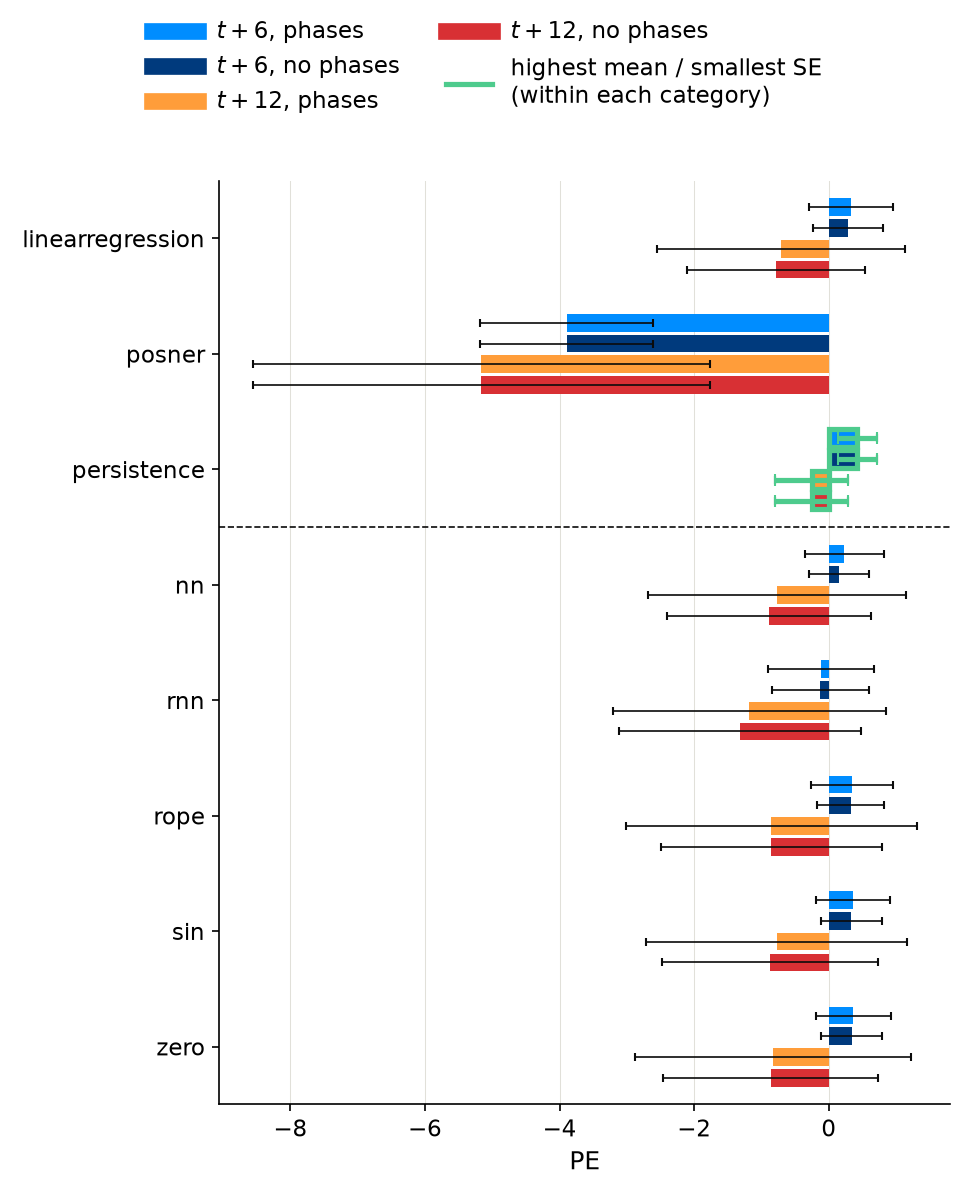
\includegraphics[width=0.7\textwidth]{figs/results/bootstrap/pe_bars_grouped.png}
    \caption{Mean prediction efficiency (PE) of every model over the 10 bootstrap datasets, one bar per forecast horizon and phase setting, with bootstrap standard error bars. Baselines are above the dashed line and champions below it. Green marks the highest mean (outline) and smallest standard error (error bar) within each category.}
    \label{fig:bootstrap_pe_bars}
\end{figure}
For ($t+6$, phases) the model with the highest PE of XXXX is from model XXXXXX with a standard error of XXXXX. YYYYY had the lowest standard error of YYYYY.
($t+6$, no-phases) model with the highest mean PE was YYY with smallest stanard error model YYY.
($t+12$, phases) highest mean PE is ZZZ with smallest standard error ZZZ
($t+12$, no-phases) highest mean PE is WWW with smallest standard error WWW
\textit{Stuff here on why i think the winning models are who they are. Confirm that the NN, RNN, Posner, Persistent models matches Torres models under same parameters}

\begin{figure}[H]
    \centering
    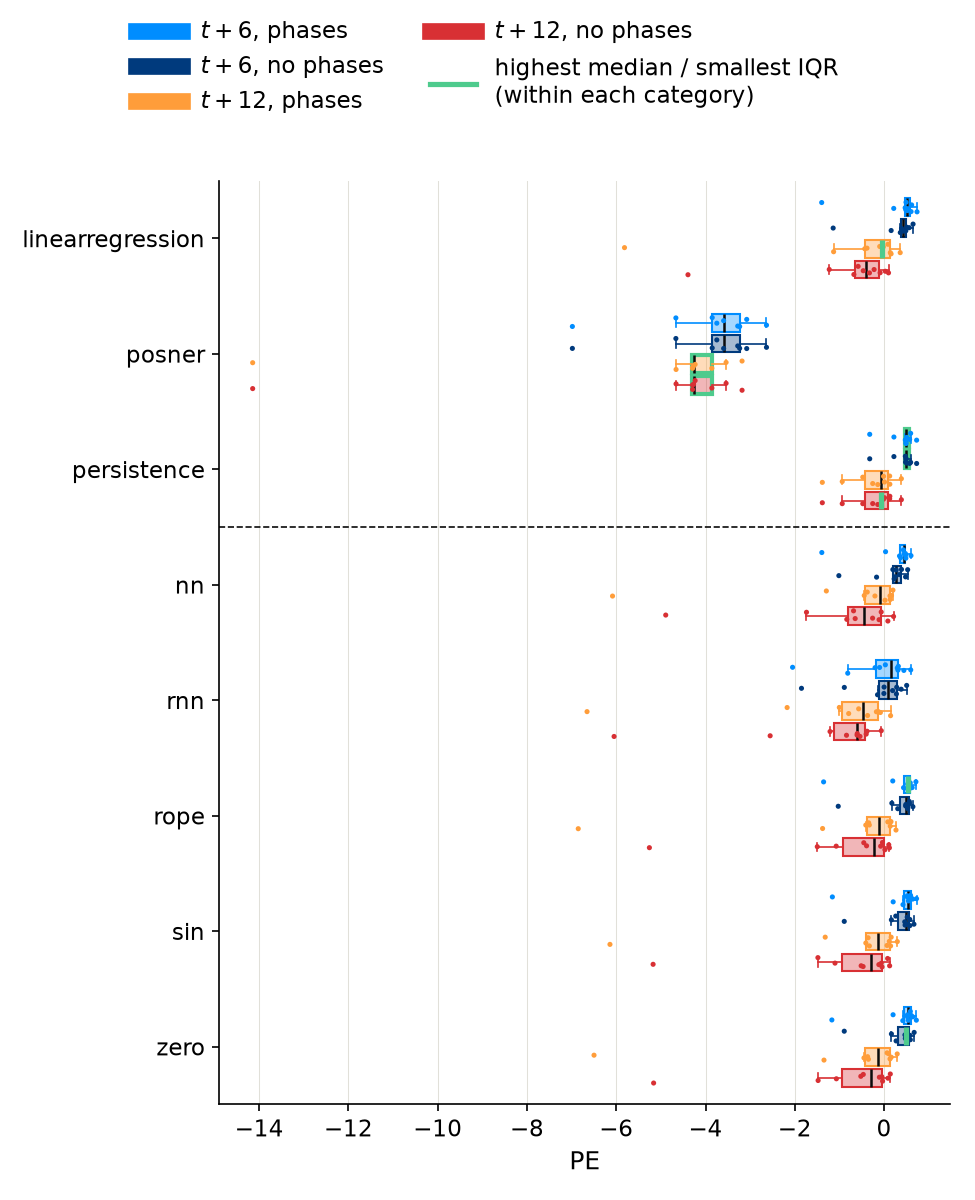
\includegraphics[width=0.7\textwidth]{figs/results/bootstrap/pe_boxplot_grouped.png}
    \caption{Prediction efficiency (PE) of every model on the 10 bootstrap datasets (seeds averaged per dataset), one box per forecast horizon and phase setting. Baselines are above the dashed line and champions below it. Green marks the highest median (line) and smallest interquartile range (box outline) within each category.}
    \label{fig:bootstrap_pe_boxplot}
\end{figure}

\subsubsection{True vs Predicted}
For each event we regress the true proton flux on each model's predicted flux, from onset to peak, and count which model has the highest $R^2$.
The fit is $\hat{y}_i = \beta_0 + \beta_1 x_i$, with $x_i$ the predicted and $y_i$ the true proton flux at time step $i$, and the 95\% prediction interval around it is
\begin{gather*}
    \text{PI}_i = \hat{y}_i \pm t_{1-\alpha/2,\,N-2}\, \sqrt{s^2 \left(1 + \frac{1}{N} + \frac{(x_i - \bar{x})^2}{S_{xx}}\right)}\\[6pt]
    s^2 = \frac{\sum_{i=1}^{N} \left(y_i - \hat{y}_i\right)^2}{N-2}, \qquad S_{xx} = \sum_{i=1}^{N} \left(x_i - \bar{x}\right)^2
\end{gather*}
where $N$ is the number of time steps from onset to peak and $\bar{x}$ is the mean predicted flux. A new true value is expected to fall inside the interval 95\% of the time.

\begin{figure}[H]
    \centering
    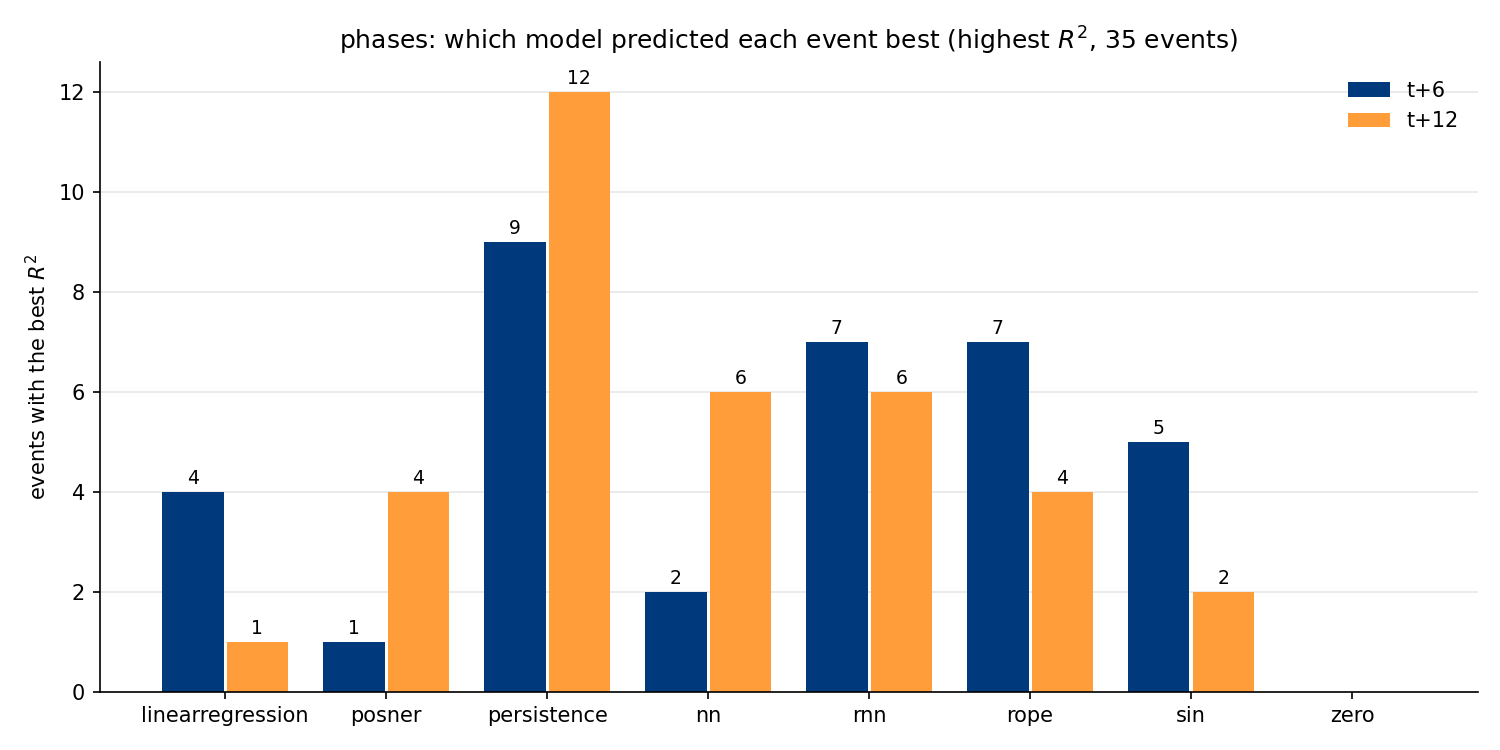
\includegraphics[width=0.7\textwidth]{figs/results/true_vs_pred/best_model_counts_phases.png}
    \caption{Number of events on which each model had the highest $R^2$ between true and predicted proton flux (onset to peak), with phases, at $t+6$ and $t+12$.}
    \label{fig:true_vs_pred_counts_phases}
\end{figure}

\begin{figure}[H]
    \centering
    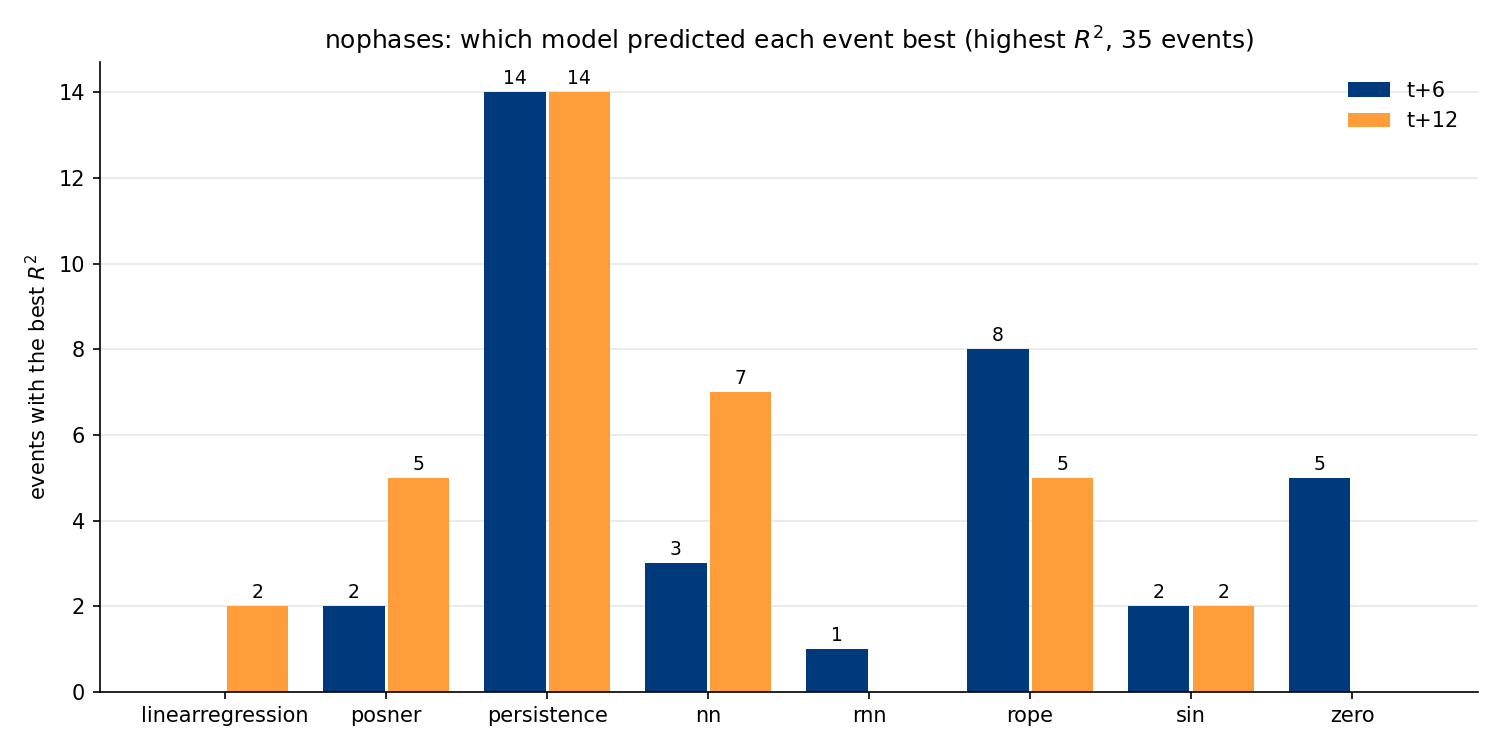
\includegraphics[width=0.7\textwidth]{figs/results/true_vs_pred/best_model_counts_nophases.png}
    \caption{Number of events on which each model had the highest $R^2$ between true and predicted proton flux (onset to peak), without phases, at $t+6$ and $t+12$.}
    \label{fig:true_vs_pred_counts_nophases}
\end{figure}

\begin{figure}[H]
    \centering
    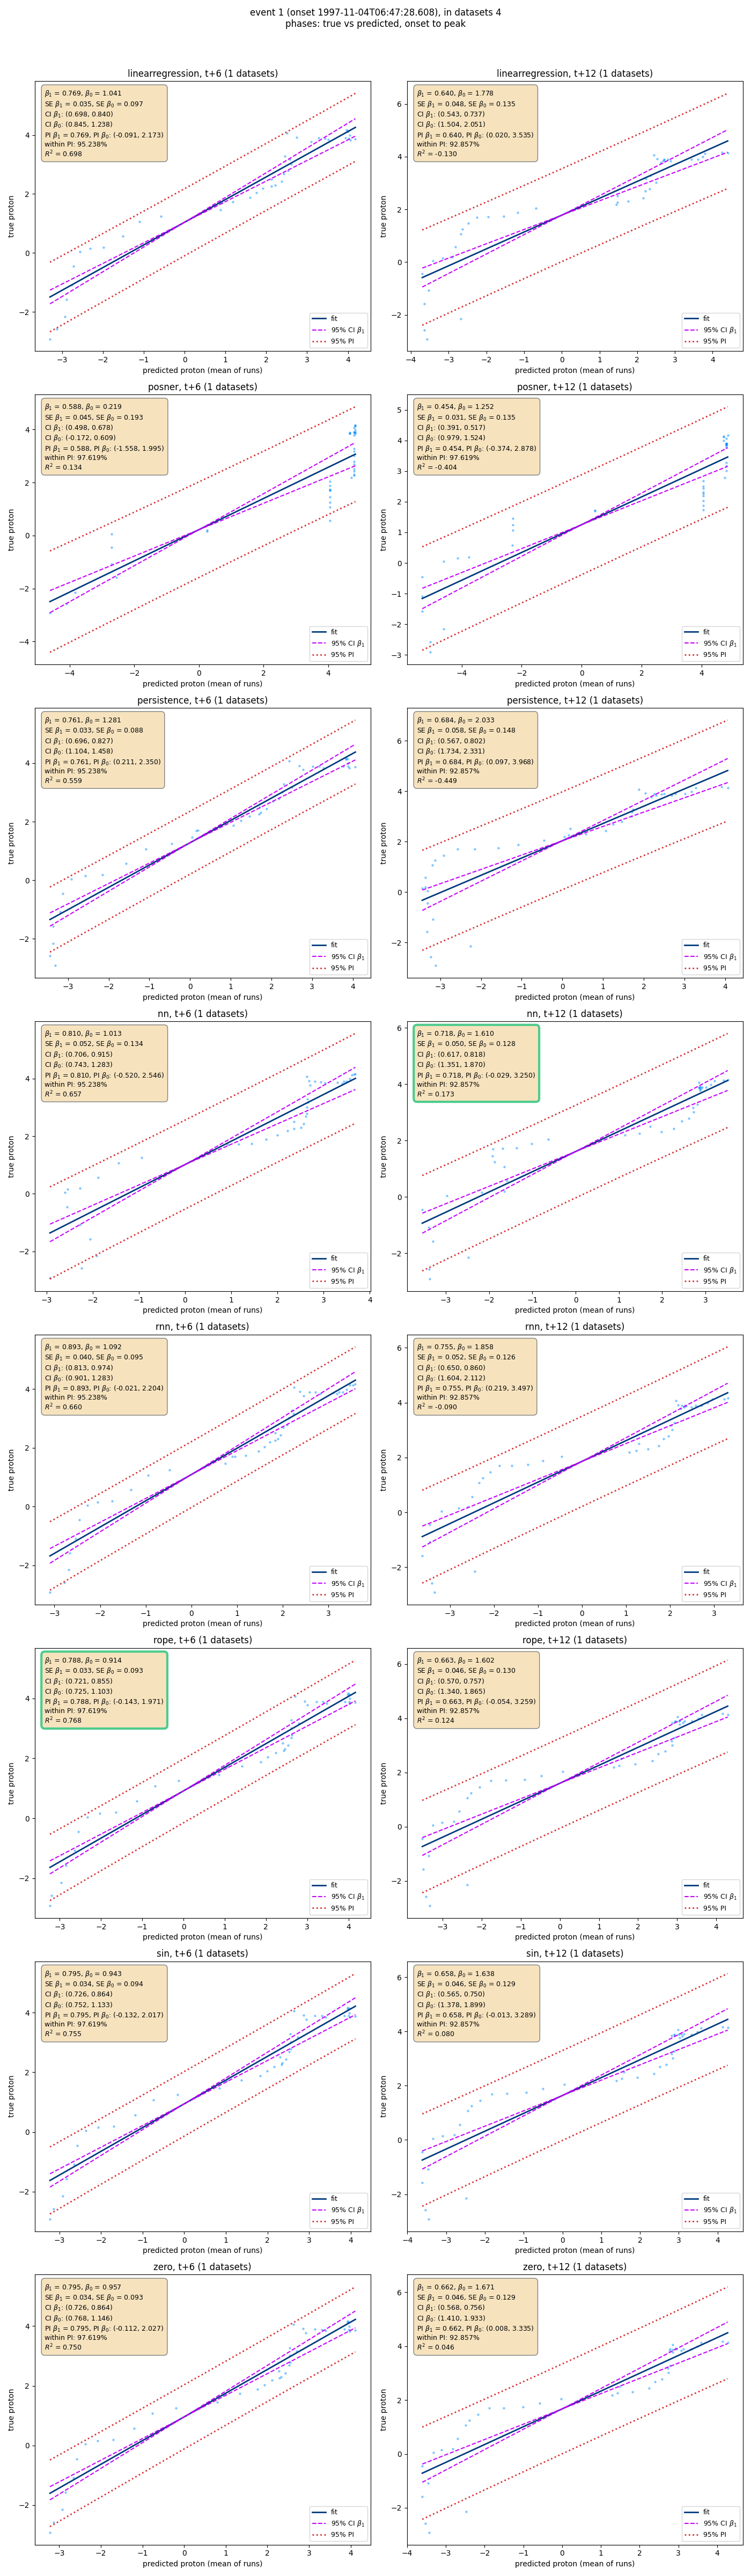
\includegraphics[height=0.85\textheight]{figs/results/true_vs_pred/event_01_phases.png}
    \caption{True vs predicted proton flux for event 1 (onset 1997-11-04), with phases: one panel per model (rows) and forecast horizon (columns), with the regression fit, the 95\% confidence interval of the slope and the 95\% prediction interval. Green boxes mark the highest $R^2$ for each horizon.}
    \label{fig:true_vs_pred_event1}
\end{figure}


\subsection{Hypothesis Testing}
\label{sec:hypothesis_testing}
We test whether each champion is better than each baseline within every category, using the one-sided Welch's $t$-test \cite{welch1947generalization} on the per-dataset means and the one-sided Levene's test with the median centre \cite{zhou2023homogeneity} on the per-dataset spread, both at $\alpha = 0.05$.
For the lags the Welch's $t$-test compares the distance from zero, $|\text{lag}|$.
Rejecting $H_0$ means the champion has the better mean (Welch) or the smaller spread (Levene).
Below are the results for the sinusoidal transformer.

\begin{figure}[H]
    \centering
    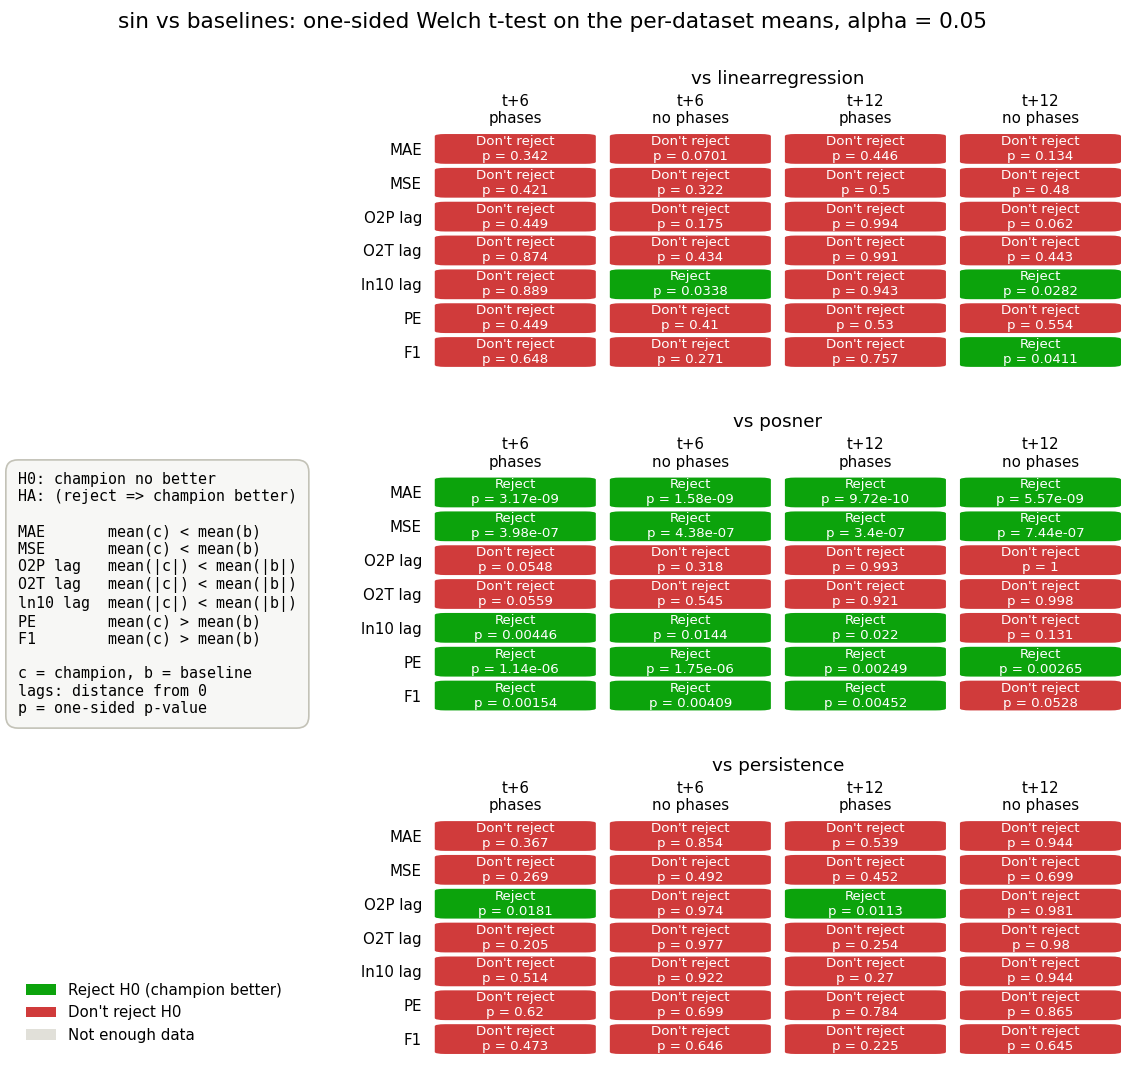
\includegraphics[width=\textwidth]{figs/results/hypothesis_testing/welch_sin.png}
    \caption{One-sided Welch's $t$-test of the sinusoidal transformer against each baseline, for every metric and category, on the per-dataset means. Green: $H_0$ rejected (sinusoidal transformer better); red: not rejected. Each cell gives the one-sided $p$-value.}
    \label{fig:welch_sin}
\end{figure}
Against XXXX the sinusoidal transformer has a significantly better mean in XXXX, while against YYYY it is not significantly better in any metric except YYYY.
\textit{Stuff here on why the sinusoidal transformer does or does not beat each baseline.}

\begin{figure}[H]
    \centering
    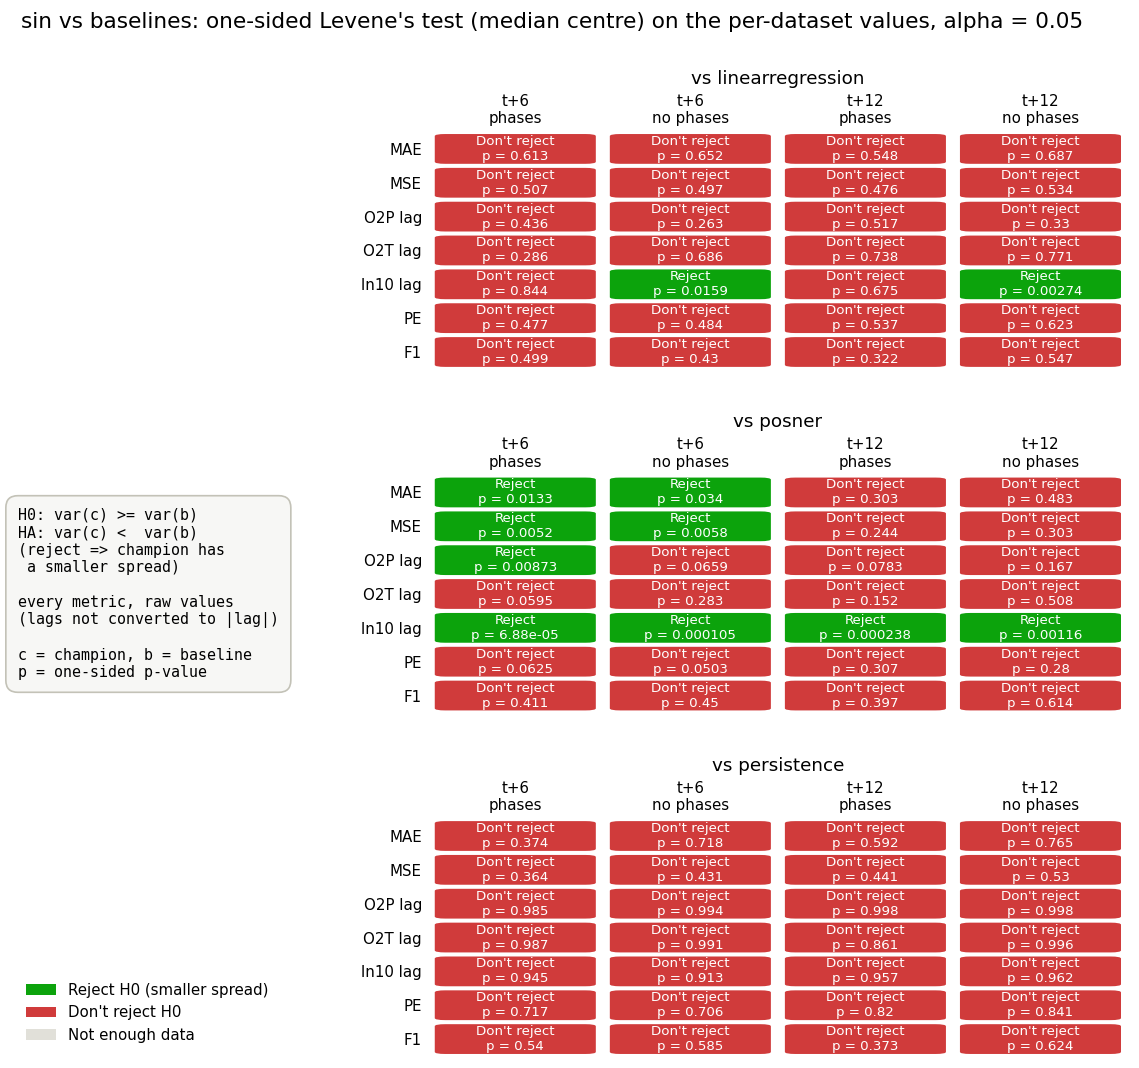
\includegraphics[width=\textwidth]{figs/results/hypothesis_testing/levene_sin.png}
    \caption{One-sided Levene's test (median centre) of the sinusoidal transformer against each baseline, for every metric and category, on the per-dataset values. Green: $H_0$ rejected (sinusoidal transformer has a smaller spread); red: not rejected. Each cell gives the one-sided $p$-value.}
    \label{fig:levene_sin}
\end{figure}
Against XXXX the sinusoidal transformer has a significantly smaller spread in XXXX, while against YYYY it is not significantly tighter in any metric except YYYY.
\textit{Stuff here on why the spread of the sinusoidal transformer is or is not smaller than each baseline.}
